% Plik jest przykładem wykorzystania klasy xmgr do formatowania 
% pracy magisterskiej.
%
% Szablon tego dokumentu można wykorzystywać formatując 
% własną pracę. Treść dokumentu nie ma specjalnie sensu i raczej
% nie nadaje się jako większy czy mniejszy fragment własnej pracy.
%
% Dostepne opcje:
%  * magisterska -- praca magisterska (wartość domyślna)
%  * licencjacka -- praca licencjacka
%  * skorowidz   -- tworzenie skorowidza
%  * xodstep     -- podwójny odstęp między wierszami
%  * brudnopis   -- zalecany na etapie  tworzenia pracy
%
\documentclass[skorowidz,brudnopis,xodstep]{xmgr}
%\documentclass[skorowidz,brudnopis,xodstep]{xmgr}

% Opcjonalnie identyfikator dokumentu (drukowany tylko 
% z włączoną opcją `brudnopis'):
\nrwersji {0.1}
%
% Przykładowe wykorzystanie pakietu fancyhdr do zdefiniowania
% tzw. żywej paginy (por. np. http://www.maths.soton.ac.uk/~ap/latex/fancyhdr.html)
%\usepackage{fancyhdr}
%\pagestyle{fancy}
%\fancyhf{}
%% 'Klasycznie', tj. wszystko w paginie górnej:
%\fancyhead[LE,RO]{\textbf{\thepage}}
%\fancyhead[LO]{\small\sffamily \nouppercase{\rightmark}}
%\fancyhead[RE]{\small\sffamily \nouppercase{\leftmark}}
%%
%\fancyfoot[LE,RO]{\textbf{\thepage}}
%\fancyhead[LE]{\small\sffamily \nouppercase{\leftmark}}
%\fancyhead[RO]{\small\sffamily \nouppercase{\rightmark}}
%%
%\renewcommand{\headrulewidth}{0.4pt}
%\renewcommand{\footrulewidth}{0.0pt}
%%

% Jeżeli nie podano szkoły zostanie wpisane na stronie tytułowej:
%     Uniwersytet Gdański -- Instytut Informatyki
%\UniversityName{Wyższa Szkoła Gdzieśtam}

%
% Dane autora(ów):
\author   {Walenty Szczęsny}
\nralbumu {rr000000001}
\email    {walenty@szczesny.com.pl}

\author   {Monika A.~Szczęsna-Woś}
\nralbumu {rr000000002}

% Tytuł pracy:
\title    {Dokumenty strukturalne: teoria i~zastosowania}

% Kierunek, tj. katedra/instytut promotora:
\kierunek {Informatyka}

% Rok obrony:
\date     {2100}

% Jeżeli nie podano miejsca zostanie wpisany `Gdańsk'
\miejsce {Gdańsk}

% Tytuł naukowy, imię i nazwisko promotora, np.:
%  dr Jan Kowalski
%  prof. dr hab.~Jan Kowalski 
% itp...
\opiekun  {prof. dr hab.~Jan Nowak}
%
% Miejsce na deklaracje własnych poleceń:
\newcommand{\filename}[1]{\texttt{#1}}

\begin{document}

% Streszczenie/Słowa kluczowe:
\begin{abstract}
  Aczkolwiek w~ciągu ostatnich lat skład tekstu wspomagany komputerowo
  całkowicie wyeliminował stosowanie tradycyjnych technik drukarskich,
  to podobny proces w~przypadku publikacji elektronicznych czyli
  publikacji, które w~ogóle nie wykorzystują papieru, a~nośnikem
  informacji staje się ekran komputera nie jest obserwowany.
\end{abstract}
\keywords{SGML, 
 XML, 
 XSL, 
 dokumenty elektroniczne, 
 dokumenty strukturalne}

% Tytuł/spis treści
\maketitle
%
% Wstęp
\introduction

Aczkolwiek w~ciągu ostatnich lat skład tekstu wspomagany
komputerowo całkowicie wyeliminował stosowanie tradycyjnych technik
drukarskich, to podobny proces w~przypadku publikacji elektronicznych
czyli publikacji, które w~ogóle nie wykorzystują papieru, a~nośnikem
informacji staje się ekran komputera nie jest obserwowany.

Formatowanie wizualne, powstało z~myślą o~przygotowaniu publikacji do
druku i~dlatego nie może sprostać nowym potrzebom, które stwarza
postęp techniki. Coraz większą rolę odgrywają dziś elektroniczne
repozytoria, bazy danych, publikacje na CD-Romach oraz WWW.  Wypływa
też stąd ważny wniosek, że tworzenie dokumentów według paradygmatu
WYSIWYG nie jest efektywne i~stopniowo należy oczekiwać powstawania,
wdrażania i~rozpowszechniania się systemów opartych na paradygmacie
\emph{formatowania strukturalnego}.

W~dokumencie formatowanym strukturalnie oznaczana jest struktura
dokumentu a~nie określany jego wygląd. Zwróćmy uwagę, że układ
graficzny jest pochodną struktury, tj. nadajemy jednolity wygląd
tytułom rozdziałów, śródtytułów, przypisów, jednakowo wyróżniamy
wyliczenia itp.  Układ graficzny jak już wspominano może ulegać zmianie
(np. wraz z~rozpowszechnianiem się nowych technologii wydawniczych)
ale treść i~struktura raczej nie, np. Biblia Gutenberga widziana z~tej
perspektywy nie zmieniła się wcale.

% Na końcu tytułów, śródtytułów, tytułów rysunków i tabel
% _nie_ umieszcza się kropki
\chapter{Wprowadzenie do standardów SGML/XML}

SGML~\cite{Goldfarb} jest to \emph{metajęzyk} służący do opisywania
struktury i~zawartości dokumentów (standard ISO 8879).  Do
podstawowych zalet takiego podejścia należy: 
\begin{itemize}
\item
jest to międzynarodowy
standard dostępny na wielu platformach sprzętowo{\dywiz}systemowych;
\item
jest to
język opisu \emph{każdego\/} dokumentu, o~praktycznie nieograniczonych
możliwościach (\emph{rozszerzalność\/}) 
\item
umożliwia powtórne
wykorzystywanie dokumentów, także w sposób inny od poprzedniego
(np. tradycyjna książka i~dokument multimedialny utworzony z~tego
samego dokumentu SGML-owego).
\end{itemize}

Standard służy jedynie do opisywania logicznej struktury dokumentów,
nie determinuje ostatecznej formy prezentacji informacji, która może
być docelowo przekształcana w~najróżniejszy sposób. Dokument
zakodowany z~wykorzystaniem SGML-a może służyć jako postać wyjściowa
do formatowania tej samej informacji w~różny sposób i~prezentacji
z~użyciem różnych mediów np. w~formie drukowanej na papierze,
w~postaci hipertekstu albo tekstowej bazy danych. Pozwala to
zminimalizować koszty\index{koszty}, cały cykl wydawniczy dokonuje się
na jednym dokumencie -- pliku SGML-owym, a~nie na wielu.
    
\section{Elementy składowe systemu SGML/XML}

Standard SGML/XML to specyfikacja techniczna metajęzyka. Zaś systemem
SGML/XML nazywamy \emph{zestaw narzędzi i~środków niezbędnych do
tworzenia, składowania i~obróbki dokumentów z~wykorzystaniem tego
standardu}.  Typowy proces produkcji dokumentów w~standardzie SGML/XML
podzielony jest na kilka części. Najważniejszymi elementami tego
procesu są~\cite[s.~45--47]{maler.devel}:
    
\begin{itemize}
\item Klasyfikacja tworzonych dokumentów w~grupy i~wynikający z~tego
  dobór definicji typu dokumentu\footnote{Definicja typu dokumentu DTD
    to formalny opis pewnej klasy dokumentów, spis jej elementów
    składowych (znaczników i~ich atrybutów) oraz zasad ich stosowania
    (hierarchii występowania czy możliwości skracania).}
  (por.~punkt~\ref{s:dtd}).
\item Wybraniu odpowiednich narzędzi do tworzenia i~modyfikowania
  dokumentów SGML/XML (edytory, konwertery, por.~punkt~\ref{s:edytor},
  s.~\pageref{s:edytor})\footnote{Wybrany edytor winien w~maksymalnym
    stopniu ułatwiać proces tworzenie dokumentów strukturalnych,
    różniący się od tego, jaki jest stosowany w~narzędziach biurowych
    typu edytor Word.}.
\item Sprawdzenie poprawności oznaczenia dokumentów
  (walidacja\index{walidacja}).
\item Ustalenie metod składowania zbiorów oznakowanych dokumentów.
\item Ustalenie sposobu prezentacji oznaczonych dokumentów i~ich
  formatów wyjściowych -- przygotowanie odpowiednich specyfikacji
  konwersji formatów i~dobór właściwych do tego celu narzędzi
  (por.~punkty~\ref{s:dsssl} i~\ref{s:xsl}).
\end{itemize}

Każdy z~wyżej wymienionych problemów stanowi pewne zadanie do
wykonania, które może być w dużym stopniu lub całkowicie
zautomatyzowane dzięki zastosowaniu odpowiednich narzędzi, co jest
jednym z~celów i~korzyści stosowania systemu opartego na standardzie
SGML/XML.

\begin{figure}[!tbh]
\centering 
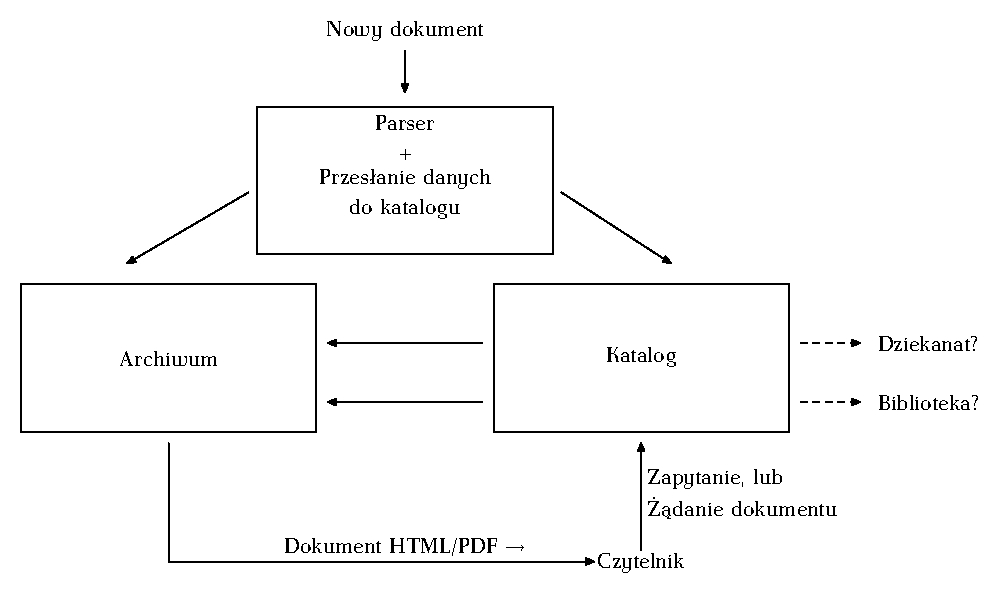
\includegraphics[width=.8\hsize]{schemat}
\caption{Schemat archiwum\label{RYS.2}}
\source{Opracowanie własne}
\end{figure}

\section{Opracowanie typu dokumentu\label{s:dtd}}
Tworzenie DTD~\cite{maler.devel,maler.ex,db.guide} powinno zacząć się
od analizy posiadanych danych oraz potrzeb dotyczących dokumentów
wynikowych i~informacji. Rezultatem analizy dokumentów jest
wyspecyfikowanie słownika takich elementów oraz, dla każdego typu
dokumentu, zależności między tymi elementami. Z~tego powodu stworzenie
dobrego DTD jest zadaniem niełatwym. Ponadto DTD jest tylko częścią
systemu SGML/XML; oprócz niego potrzebne są narzędzia do formatowania
dokumentów, takie jak arkusze stylów DSSSL czy też XSL/XSLT.
    
Duże koszty implementacji przemawiają często za rozważeniem
wykorzystania, czy też adaptacji w~systemie SGML/XML udostępnionych
publicznie gotowych DTD. W~omawianym projekcie postąpiono podobnie,
ewentualne opracowanie własnego typu dokumentu odkładając na później.
Rozważano wstępnie wykorzystanie trzech publicznie dostępnych typów
dokumentów: \texttt{etd} zdefiniowanego na potrzeby projektu
\textit{Electronic Theses and Dissertations} w~Virginia Polytechnic
Institute and State University, \texttt{TEI} opracowanego w~ramach
projektu \textit{Text Encoding Iniciative} \cite{tei.intro} oraz
DocBook opracowany przez konsorcjum firm, głównie sektora IT,
używających technologii SGML/XML do tworzenia dokumentacji do swoich
produktów~\cite{db.guide}.
    
\section{DocBook}
\emph{DocBook DTD}\index{DocBook|(} to typ dokumentu definiujący
strukturę i~zawartość zbioru znaczników SGML, służących do
dokumentacji oprogramowania i~różnego rodzaju dokumentacje
techniczne~\cite[s.~123]{db.guide}. Posiada ona bardzo rozbudowaną
hierarchię znaczników do budowy struktur książek, dokumentacji
technicznej itp dokumentów.  DTD dla tego typu dokumentu jest dostępne
zarówno w~standardzie SGML jak i~XML. Dostępna jest także uproszczona
wersja DTD o~nazwie SimpleDocbook. Zaletą używania wersji uproszczonej
jest dużo łatwiejsze posługiwanie się nią, z~uwagi na znacznie
mniejszą liczbę znaczników, por.~tabela~\ref{tab:dtd-cmp}.

\begin{table}[!tbh]
\begin{tabular}{|l|l|l|} \hline
Typ dokumentu & Liczba elementów & Liczba encji \\ \hline
Docbook & 357 & 1814 \\ \hline
SimpleDocBook  & 93  & 234 \\ \hline
TEI & brak danych & 3 \\ \hline
HTML & 98  & 234 \\ \hline
\end{tabular}
\caption{Porównanie wielkości popularnych definicji 
  typu dokumentu\label{tab:dtd-cmp}}
\source{Obliczenia własne}
\end{table}

DocBook jest używany obecnie w~większości zarówno komercyjnych jak
i~niekomercyjnych projektach tworzenia dokumentacji komputerowej
(np. dokumentacja dla takich projektów jak: LDP -- \textit{Linux
Documentation Project}, \textit{RedHat Gnome Desktop},
\textit{Postgres SQL RDBMS}, \textit{PHP3 Hypertext Preprocesor} czy
dokumentacja do systemu FreeBSD).\index{DocBook|)}
    
\section{Edytory sterowane składnią\label{s:edytor}}

Pierwszym elementem systemu SGML/XML jest edytor
strukturalny\index{edytor!strukturalny}, zwany też edytorem sterowanym
składnią. W~tradycyjnych edytorach działających według paradygmatu
WYSIWYG\index{WYSIWYG} autor wprowadzając tekst określa na bieżąco
jego wygląd, mając zarówno w~jednym jak i~drugim przypadku dużą
swobodę.  Taki sposób pracy w~przypadku masowego tworzenia dokumentów
jest zupełnie nieefektywny. W~szczególności dotyczy to pracy wielu
autorów nad jednym lub wieloma dokumentami o~zuniformizowanym
formacie, czy też tworzenia dokumentów, o~których z~góry wiadomo, że
będą prezentowane w~różny sposób.

Pewnym rozwiązaniem opisywanych wyżej problemów jest wykorzystanie
szablonów, w~które, od jakiegoś czasu są wyposażane wszystkie
popularne edytory biurowe\index{edytor!biurowy}.  Posługując się
szablonami, autor nie definiuje wyglądu samodzielnie tylko wypełnia
treścią zdefiniowany z~góry szablon dokumentu.  
Stanowiąc niewątpliwy
krok do przodu takie podejście nie rozwiązuje jednak wszystkich
problemów.

Komercyjne edytory SGML, są w~chwili obecnej ciągle bardzo
drogie, zaś oprogramowanie rozprowadzane na różnego rodzaju licencjach
\emph{Open Source\/} nie oferuje jeszcze wygody pracy, do której
przyzwyczaili się użytkownicy edytorów biurowych.  

\section{Emacs i~psgml}

Konstatując brak tanich i~funkcjonalnych edytorów do pracy
z~dokumentami SGML/XML należy wspomnieć o~jedynym dostępnym w~chwili
obecnej, efektywnym, tanim (darmowy) i~powszechnie dostępnym na wielu
platformach systemowo-sprzętowych środowisku do tworzenia dokumentów
strukturalnych jakim jest edytor Emacs\index{edytor!Emacs} z~pakietem
psgml. Środowisko to wspomaga autora poprzez:
kolorowanie składni dokumentów SGML i~aplikacji SGML, automatyczne
uzupełnianie brakujących znaczników, automatyczną kontrolę jakie
w~danym kontekście można wstawiać znaczniki i~atrybuty, wyświetlanie
informacje odnośnie możliwych i~domyślnych wartości. 
Wszystkie funkcje są dostępne za pomocą
odpowiednie skrótów klawiszowych a~także dostępne poprzez wybór
wskaźnikiem myszy odpowiedniej pozycji z~menu. Pakiet ten umożliwia
również wywołanie zewnętrznego parsera\index{parser} SGML celem
weryfikacji poprawności dokumentu.
      
\chapter{Narzędzia i~standardy pokrewne}

Systemy SGML, ze względu na mnogość funkcji jakie spełniają i~ich
kompleksowe podejście do oznakowywania i~przetwarzania dokumentów
tekstowych, są bardzo skomplikowane. Możemy wyróżnić dwa podejścia do
budowy takich systemów.  Z~jednej strony, buduje się systemy
zindywidualizowane, oparte o~specyficzne narzędzia tworzone w~takich
językach, jak: C, C++, Perl czy Python. Edytory strukturalne, filtry
do transformacji formatów czy parsery\index{parser} i~biblioteki
przydatne do konstrukcji dalszych narzędzi, tworzone są według potrzeb
określonych, pojedynczych systemów.
    
Z~drugiej strony, twórcy oprogramowania postanowili pójść krok dalej
i~połączyć te różne narzędzia w~jedną całość. Tą całość miał stanowić
DSSSL lub jego XML-owy odpowiednik -- standard XSL. Ze względu na
oferowane możliwości można twierdzić, że tworzenie i~używanie narzędzi
implementujących standard DSSSL/XSL, jest najwłaściwszym
podejściem. Przemawiają za tym różne argumenty, ale najważniejszym
z~nich jest to, że mamy tu możliwość stworzenia niezależnego od
platformy programowej i~narzędziowej zbioru szablonów -- przepisów jak
przetwarzać dokumenty SGML/XML.
    
\section{Przetwarzanie dokumentów SGML -- standard DSSSL\label{s:dsssl}}

DSSSL (\textit{Document Style Semantics and Specification Language\/})
-- to międzynarodowy standard ściśle związany ze standardem SGML.
Standard ten, można podzielić na następujące części:

\begin{itemize}
\item język transformacji (\textit{transformation language\/}).  To
  definicja języka służącego do transformacji dokumentu oznaczonego
  znacznikami zgodnie z~pewnym DTD na dokument oznaczony zgodnie
  z~innym~DTD.
\item język stylu (\textit{style language\/}) opisujący sposób
  formatowania dokumentów SGML.
\item język zapytań (\textit{query language\/}) służy do
  identyfikowania poszczególnych fragmentów dokumentu SGML.
\end{itemize}

Opisane główne części składowe standardu DSSSL dają obraz tego, jak
wiele aspektów przetwarzania zostało zdefiniowanych i~jak
skomplikowany jest to problem. Jest to głównym powodem tego, że mimo
upływu kilku lat od zdefiniowania standardu nie powstały ani
komercyjne ani wolnodostępne aplikacje wspierające go
w~całości. Istnieją natomiast \emph{nieliczne\/} narzędzia realizujące
DSSSL w~ograniczonym zakresie, głównie w~części definiującej język
stylu, który odpowiada za opatrzenie dokumentu czysto strukturalnego
w~informacje formatujące. Daje to możliwość publikacji dokumentów SGML
zarówno w~postaci elektronicznej, hipertekstowej czy też drukowanej.
      
\section{Przetwarzanie dokumentów XML -- standard XSL\label{s:xsl}}

Tak jak XML jest \emph{uproszczoną\/} wersją standardu SGML, tak XSL
jest uproszczonym odpowiednikiem standardu DSSSL. W~szczególności,
wyróżnić można w~tym standardzie następujące części składowe:

\begin{itemize}
\item język transformacji (XSLT) To definicja języka służącego do
  transformacji dokumentu.      
\item język zapytań (XPath) służy do identyfikowania poszczególnych
  fragmentów dokumentu.
\item język stylu deefiniujący sposób formatowania dokumentów XML.
\end{itemize}

\chapter{Przegląd dostępnych narzędzi\label{PRZEGLAD.NARZEDZI}}

W~celu wykorzystania standardu SGML/XML do przetwarzania dokumentów,
niezbędne jest zebranie odpowiedniego zestawu narzędzi. Narzędzi do
przetwarzania dokumentów SGML/XML jest wiele. Są to zarówno całe
systemy zintegrowane, jak i~poszczególne programy, biblioteki czy
skrypty wspomagające.
    
\section{Narzędzia do przeglądania dokumentów SGML/XML}

Do tej kategorii oprogramowania zaliczamy przeglądarki dokumentów
SGML/XML oraz serwery sieciowe wspomagające standard SGML/XML, przy
czym rozwiązań wspierających standard XML jest już w~chwili obecnej
dużo więcej i~są dużo powszechniejsze.

Jeżeli chodzi o~przeglądarki to zarówno Internet Explorer jak
i~Netscape umożliwiają bezpośrednie wyświetlenie dokumentów XML;
ponieważ jednak nie wspierają w~całości standardu XML, prowadzi to
ciągle do wielu problemów\footnote{Z~innych mniej popularnych
  rozwiązań można wymienić takie aplikacje, jak: HyBrick SGML/XML
  Browser firmy Fujitsu Limited, Panorama Publisher firmy InterLeaf
  Inc, DynaText firmy Inso Corporation czy darmowy QWeb. W~przypadku
  serwerów zwykle dokonują one transformacji ,,w~locie'' żądanych
  dokumentów na format HTML (rzadziej bezpośrednio wyświetlają
  dokumenty XML).  Ta kategoria oprogramowania ma, z~punktu widzenia
  projektu, znaczenie drugorzędne.}.
      
\section{Parsery SGML/XML}
Program \texttt{nsgmls} (z~pakietu \texttt{SP} Jamesa Clarka) jest
doskonałym parserem\index{parser} dokumentów SGML, dostępnym
publicznie.  Parser \texttt{nsgmls} jest dostępny w~postaci źródłowej
oraz w~postaci programów wykonywalnych przygotowanych na platformę
MS~Windows, Linux/Unix i~inne. Oprócz analizy poprawności dokumentu
parser\index{parser} ten umożliwia również konwersję danych do formatu
ESIS\index{ESIS}, który wykorzystywany jest jako dane wejściowe przez
wiele narzędzi do przetwarzania i~formatowania dokumentów SGML.
Dodatkowymi, bardzo przydatnymi elementami pakietu \texttt{SP} są:
program \texttt{sgmlnorm} do normalizacji, program \texttt{sx} służący
do konwersji dokumentu SGML na XML oraz biblioteki programistyczne,
przydatne przy tworzeniu specjalistycznych aplikacji służących do
przetwarzania dokumentów SGML.
      
W~przypadku dokumentów XML publicznie dostępnych, parserów jest
w~chwili obecnej kilkadziesiąt. Do popularniejszych zaliczyć można
Microsoft Java XML Parser firmy Microsoft, LT XML firmy Language
Technology Group, Exapt oraz XP (James Clark)
      
\section{Wykorzystanie języków skryptowych}
      
\section{Wykorzystanie szablonów XSL}

Stosując wersję XML typu DocBook można wykorzystać szablony stylów
przygotowane w~standardzie XSL (autor N.~Walsh). W~chwili obecnej
są dostępne narzędzia umożliwiające przetworzenie dokumentów XML do
postaci drukowanej (Adobe PDF) oraz hipertekstowej (HTML).

Podobnie jak w~przypadku szablonów DSSSL, szablony stylów XSL są
sparametryzowane i~udokumentowane i~dzięki temu łatwe w~adaptacji. Do
zamiany dokumentu XML na postać prezentacyjną można wykorzystać jeden
z~dostępnych publicznie procesorów XSLT
(por.~tabela~\ref{zest:proces:xslt}).

\begin{table}[!htb]
\begin{tabular}{|l|l|l|} \hline
Nazwa & Autor      & Adres URL \\ \hline
\texttt{sablotron} & Ginger Alliance & \url{http://www.gingerall.com} \\ \hline
\texttt{Xt}        & J.~Clark & \url{http://www.jclark.com} \\ \hline
\texttt{4XSLT}     & FourThought & \url{http://www.fourthought.com} \\ \hline
\texttt{Saxon}     & Michael Kay &  \url{http://users.iclway.co.uk/mhkay/saxon} \\ \hline
\texttt{Xalan}     & Apache XML Project & \url{http://xml.apache.org} \\ \hline
\end{tabular}
\caption{Publicznie dostępne procesory XLST\label{zest:proces:xslt}}
\source{Opracowanie własne}
\end{table}

Wykorzystując szablony, na podstawie dokumentu XML otrzymujemy
bezpośrednio dokument HTML. W~przypadku wersji drukowanych sprawa jest
bardziej skomplikowana (por.~rys.~\ref{fig:xsl-fo}).

\begin{figure}[!tbh]
\centering 
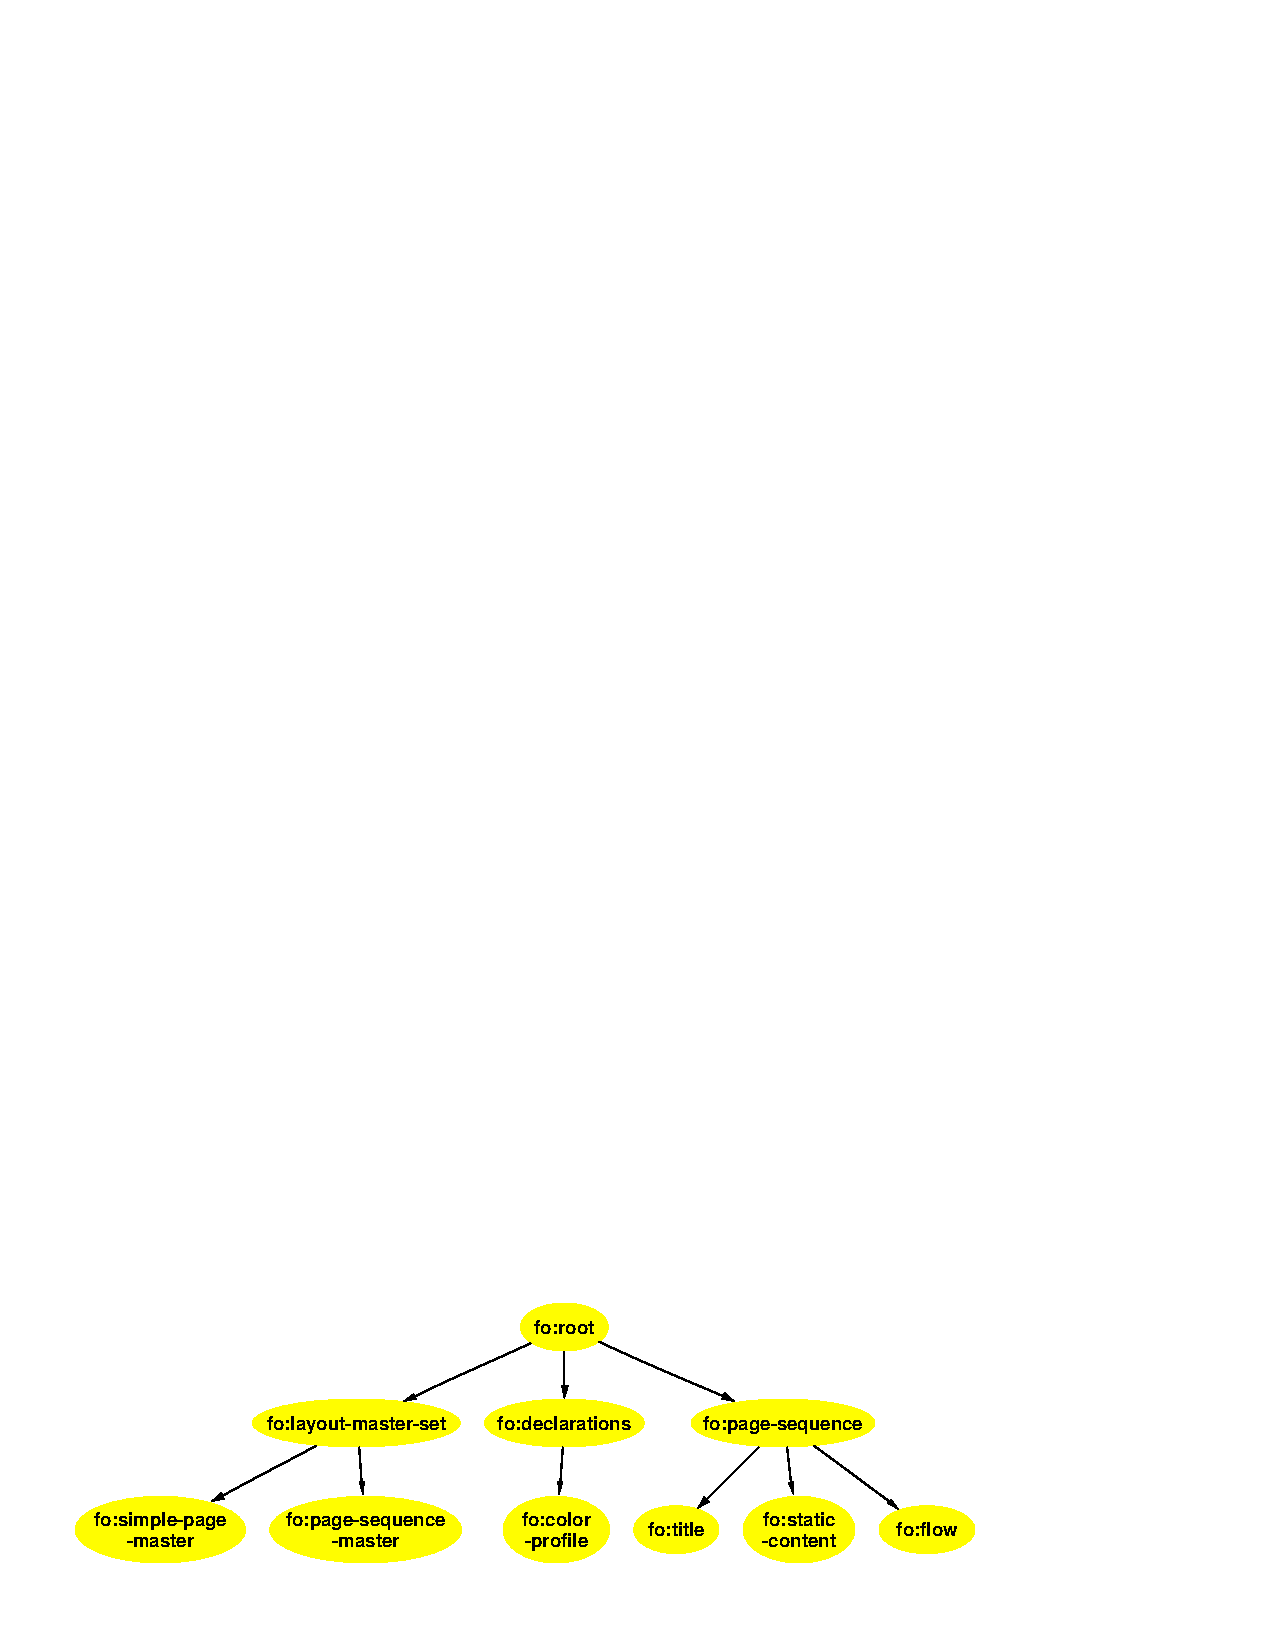
\includegraphics[width=.8\hsize]{fo-structure}
\caption{Ogólna struktura dokumenu XSL-FO\label{fig:xsl-fo}}
\source {Opracowanie własne}
\end{figure}

XSL:FO jest skomplikowanym językiem o~dużych możliwościach,
zawierającym ponad 50 różnych ,,obiektów formatujących'', począwszy od
najprostszych, takich jak prostokątne bloki tekstu poprzez wyliczenia,
tabele i~odsyłacze. Obiekty te można formatować wykorzystując przeszło
200 różnych właściwości (\emph{properties\/}), takich jak: kroje,
odmiany i~wielkości pisma, odstępy, kolory itp.  
W~tym dokumencie przedstawione jest absolutne miniumum informacji 
na temat standardu XSL:FO.

Cały dokument XSL:FO zawarty jest wewnątrz elementu \texttt{fo:root}.
Element ten zawiera (w~podanej niżej kolejności):
 %
\begin{itemize}
\item dokładnie jeden element \texttt{fo:layout-master-set} zawierający
  szablony określające wygląd poszczególnych stron oraz sekwencji
  stron (te ostatnie są opcjonalne, ale typowo są definiowane);
\item zero lub więcej elementów \texttt{fo:declarations};
\item jeden lub więcej elementów \texttt{fo:page-sequance}
 zawierających treść formatowanego dokumentu wraz z~opisem
 jego sformatowania i~podziału na strony.
\end{itemize}

%
% Zakończenie 
\summary
Możliwości, jakie stoją przed archiwum prac magisterskich opartych na
XML-u, są ograniczone jedynie czasem, jaki należy poświęcić na pełną
implementację systemu. Nie ma przeszkód technologicznych do stworzenia
co najmniej równie doskonałego repozytorium, jak ma to miejsce w
przypadku ETD. Jeżeli chcemy w pełni uczestniczyć w rozwoju nowej ery
informacji, musimy szczególną uwagę przykładać do odpowiedniej
klasyfikacji i archiwizacji danych. Sądzę, że język XML znacznie to
upraszcza.

%
% Załączniki (opcjonalnie):
\appendix
\chapter{Tytuł załącznika jeden}

Treść załącznika jeden. Treść załącznika jeden. Treść załącznika jeden
Treść załącznika jeden. Treść załącznika jeden.
Treść załącznika jeden.

\chapter{Tytuł załącznika dwa}

Treść załącznika dwa. Treść załącznika dwa. Treść załącznika dwa
Treść załącznika dwa. Treść załącznika dwa.
Treść załącznika dwa.

%
% Literatura (obowiązkowo):
\begin{thebibliography}{99}
% Pozycja bibliograficzna typu: książka.
% autor/autorzy: tytuł, wydawca, rok-wydania
\bibitem{tei.intro}
Burnard L.,
Sperberg-McQueen C. M.:
\textit{TEI Lite: An Introduction to Text Encoding for Interchange},
1995.
\url{http://www.uic.edu/orgs/tei/intros/teiu5.html}.

% Czasami zamiast autora-osoby należy umieścić nazwę organizacji/firmy,
% tak jak w przykładzie poniżej
\bibitem{pdf.spec}
Adobe Systems Inc:
\textit{Portable Document Format Reference Manual Version 1.2},
Addison-Wesley, 1996.

% Pozycja bibliograficzna typu: artykuł.
% autor/autorzy: ,,tytuł-artykułu'', tytuł-czasopisma numer, rok, strony
\bibitem{beebe}
Beebe N.~H.~F.:
,,Bibliography Prettyprinting and Syntax Checking'',
\textit{TUGBoat} 14/4, 1995, 
s.~395--419.

% Pozycja bibliograficzna typu: rozdział z pracy zbiorowej/monografii.
% autor/autorzy: ,,tytuł-rozdziału'', w: tytuł-książki
%   (red. redaktor), miejsce-wydania rok-wydania, strony
\bibitem{}
Braams J. L.:
The Status of Babel,
w:~\textit{Proceedings of the IXth European TeX Conference}
(W. Dol red.), Arnhem 1995, s.~17--26.

\bibitem{XMLspec}
Bray T.,
Paoli J.,
Sperberg-McQueen C.~M.:
\textit{Extensible Markup Language (XML)~1.0},
1998. \url{http://www.w3.org/TR/1998/REC-xml-19980210}.

\bibitem{bryan}
Bryan M.:
\textit{SGML and HTML explained},
Addison-Wesley
1997.

\bibitem{xslt}
Clark J.:
\textit{XSL Transformations (XSLT) Version~1.0},
1999. \url{http://www.w3.org/TR/xslt}.

\bibitem{p.flynn}
Flynn P.:
\textit{Understanding SGML and XML tools},
Kluwer Academic Publishers
1998.

\bibitem{Goldfarb}
Goldfarb C.:
\textit{The SGML Handbook},
Oxford University Press.

\bibitem{lwc}
Goossens M.,
Rahtz S.:
\textit{The {\LaTeX} Web Companion},
Addison-Wesley
1999.

\bibitem{python.tkinter}
Grayson J.:
\textit{Python and Tkinter programming},
Manning Publications.

\bibitem{Herwinen-Pract}
Van Herwijnen E.:
\textit{Practical SGML},
Kluwer Academic Publishers
1990.

\bibitem{lamport}
Lamport L.:
\textit{{\LaTeX}: a~document preparation system},
Addison-Wesley
1994.

\bibitem{maler.ex}
Maler E.:
\textit{SGML exceptions and XML},
1998.
\url{http://www.arbortext.com/Think_Tank/XML_Resources/SGML_Exceptions_and_XML}.

\bibitem{maler.devel}
Maler E.,
El Andaloussi J.:
\textit{Developing SGML DTDs. From Text to Model to Markup},
Prentice Hall
1996.

\bibitem{s.north}
North S.:
\textit{XML dla każdego},
Helion
2000.

\bibitem{whirlwind-guide}
Pepper S.:
\textit{Whirlwind Guide to SGML Tools and Vendors}.
\url{http://www.infotek.no/sgmltool/index.htm}.

\bibitem{p.perl}
Wall L.,
Christiansen T.,
Schwartz R.:
\textit{Programming Perl},
O'Reilly \&~Associates
1996.

\bibitem{db.guide}
Walsh N.,
Muellner L.:
\textit{DocBook: The Definitive Guide},
O'Reilly \&~Associates October~1999.
Dokument dostępny także w~\url{http://www.docbook.org/}.

\end{thebibliography}

%
% Spis tabel (jeżeli jest potrzebny):
\listoftables
%
% Spis rysunków (jeżeli jest potrzebny):
\listoffigures

%
% Skorowidz (opcjonalnie)
%\printindex

\oswiadczenie

\end{document}
